\subsection{Create zero sales}\label{zerosales}

The training dataset tells us exactly which item got sold when and where. At the same time, this tells us exactly which shop did not sell any item on a given date.
With this information, we can craft the possibly most important feature of them all: add the records from a possible combination of a given month, all shops and all items. Then fill the sale record with 0. This operation was dubbed \enquote{create zero sales}.
The mathematical function of this operation can be expressed with the following cartesian product:

\vspace*{-4mm}
$$
\{\text{\texttt{date\_block\_num}}_i\}
\quad \times \quad
\{{\text{\texttt{shop\_id}}}\}
\quad  \times \quad 
\{{\text{\texttt{item\_id}}}\}
\quad \mid \quad
i \cap [0; 33], \quad i \in \mathbb{N}
$$

This operation was implemented using the Python function \texttt{product} from the \texttt{itertools} package from the Python standard library.\footnote{\href{https://docs.python.org/3/library/itertools.html\#itertools.product}{\texttt{itertools} - official documentation}}

\noindent \textit{N.B. that this ignores the months which have not sold anything in the considered time period.}

\subsection{Shop information}

To add detailed information about the shops, we first identified the city in which a shop is located. To continue from there, we researched geographic and demographic data. This information was added to a spreadsheet and exported as \acrfull{csv} file in a similar manner to the original dataset. The following features have been added: \texttt{zip\_code}, \texttt{region}, \texttt{population}, \texttt{population\_growth} and \texttt{region\_gdp}.

The population growth was considered, on a city level, from a time frame roughly between 2010--2018 (varying according to different sources from discovered materials).

The population and gdp (per capita) information were primarily taken from the year 2018. Again, this was due to the abundance of information publicly available for this period.

\subsection{Category information}

Compared to the shop information, the process of arranging detailed features for the various categories was relatively arbitrary. After translating all 84 categories, some were very specific and hereby intuitive, for instance the category 12 \enquote{Game consoles - PS4}. This could easily be split into a type (\enquote{game console}), a dedicated device (\enquote{ps4}), platform (\enquote{playstation}), manufacturer (\enquote{sony}) and a medium (\enquote{physical}).

The same distinctions were harder to make for other categories like \enquote{Gifts - Stuffed Toys} or \enquote{Service}. As these can be interpreted very differently, we attempted to create meaningful splits to our best intentions. The resulting features can be found in the \acrshort{csv} file \href{\repoblobbaseurl\finalCommit/data/feature_engineering/cities.csv}{on GitHub}.

The feature \texttt{category\_is\_fancy}, evolved from the distinction in certain existing categories like \enquote{PC Games - Standard Editions} and \enquote{PC Games - Collector's Editions} which expects the latter to have a narrower target audience for a same title.

\subsection{Lag features}

\begin{wrapfigure}[8]{l}{0.48\textwidth}
\centering
\newcommand{\putrow}[3]{
\path (0,#1) node{#2} ++(0:1) node{#3};
}

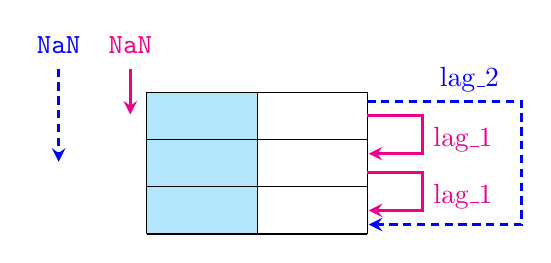
\begin{tikzpicture}[xscale=1.4,yscale=.6]
\begin{scope}[shift={(-.5,.5)}]
\fill[cyan!30] (0,0) rectangle +(1,-3);
\draw (0,0) grid (2,-3);
\end{scope}

\begin{scope}[-stealth,magenta,shorten >=.5pt,
every node/.style={midway,scale=1}]
\draw[line width=0.4mm] (1.5,0)--(2,0)--(2,-0.8)--(1.5, -0.8)    node[right, xshift=10, yshift=5]{lag\_1};
\draw[line width=0.4mm] (1.5,-1.2)--(2,-1.2)--(2,-2)--(1.5, -2)    node[right, xshift=10, yshift=5]{lag\_1};

\draw[line width=0.4mm] (-0.65, 1)--(-0.65, 0)    node[above, yshift=10]{\texttt{NaN}};
\end{scope}

\begin{scope}[-stealth,blue,shorten >=.5pt,
every node/.style={midway,scale=1}]
\draw[line width=0.4mm][densely dashed] (1.5,0.3)--(2.9,0.3)--(2.9,-2.3)--(1.5, -2.3)    node[above, xshift=9, yshift=44]{lag\_2};

\draw[line width=0.4mm][densely dashed] (-1.3, 1)--(-1.3, -1)    node[above, yshift=18.5]{\texttt{NaN}};

\end{scope}

\putrow{0}{Apr}{5}
\putrow{-1}{May}{2}
\putrow{-2}{Jun}{4}
\end{tikzpicture}

\captionsetup{justification=centering}
\caption{Creating lag features}
\label{lag}
\end{wrapfigure}


In the next step, we have created a set of lag features. The adjoining figure \ref{lag} illustrates their implementation. 
The idea is that, in a time series, every label $y_t$, in function of its time $t$, is dependent on its preceding value $y_{t-n}$.
$n$ is chosen to suit the time interval of the problem, for instance $n \cap \{1;2;3;6;12\}$ to consider the past two months, trimester, semester and year in a monthly spaced time series. Consequently, the lag$\_n$ series shifts the label for $n$ intervals forward in time. To apply this feature on several different existing features, the following function has been implemented:

\lstinputlisting[language=python, caption=Compute Lag Features (in Python), label=lagfeatures]{external_content/code/lag_features.py}

The function seen in listing \ref{lagfeatures} receives following parameters: a \gls{df} \texttt{df}, the intervals \texttt{lags} in which the features are intended to be lagged and the features which are lagged. Then, the individual lags are iterated over: begin by storing the relevant columns from the \gls{df}, add a new column, shift the date \texttt{n} forward and merge the newly created feature back onto the passed \gls{df}.


\subsection{Price related features}

Primarily to avoid throwing the new items from the test set under the bus (identified in section \ref{sec:testdata}), a variety of average prices has been calculated. This includes the average price of a given item overall, as well as the average price an item has in each shop and the average price of items in a given category.
% TODO: as well as the average price, this given item has in each shop
This is intended to nudge the model in a certain direction.

On top of that, a trend feature has been added. This is effectively a lag of the item price. 
This indicates the direction of item prices. This accounts for the trend observed in figure \ref{fig:total_sales} and figure \ref{fig:total_revenue}, which imply fewer sales with rising item prices over time.

\subsection{Additional features}

To finish off the feature engineering, a few selected features have been crafted representing additional information gathered from the time data. A few are simple features, such as the month of the year. This is intended to take the seasonality into account. A feature which holds the number of days in a month, with intents to explain the difference in sales when having a month with 31 days or 28 days, thus having roughly 10\% more days where the shops are open for business.\footnote{Shops in Russia are generally open 7 days a week}

Another set of features, which has been a little bit trickier to implement, is the record of when an item has been initially and most recently sold on a companywide and on a given shop basis.
To achieve this, we created a set for each feature respectively, and stored a key pair \texttt{(item\_id, shop\_id)}with the resulting dates. Finally, the set has been matched to the corresponding rows in the \gls{df}.
